\documentclass[12pt]{article}
\usepackage[numbers]{natbib}
\usepackage[margin=1in]{geometry}
\usepackage[nottoc]{tocbibind}
\usepackage{graphicx}
\usepackage{svg}
\usepackage{setspace}
\graphicspath{{../out/graphs/}}

\doublespacing

\author{Thomas Kwashnak}
\title{Comparing Machine Learning Libraries to Manual Implementations}

\newcommand{\CC}{C\nolinebreak\hspace{-.05em}\raisebox{.4ex}{\tiny\bf +}\nolinebreak\hspace{-.10em}\raisebox{.4ex}{\tiny\bf +} }

\begin{document}

\maketitle

\newpage

\newpage

\section{Abstract}

Popular machine learning frameworks seek to simplify the use of complex machine learning tasks.
Frameworks such as TensorFlow allow users to utilize GPU optimizations by using abstractions.
However, these abstractions may negatively affect the performance of a model.
In this paper, we look at the performance of a feed-forward and back-propogation algorithm for neural networks, implemented on the GPU or CPU, either using the TensorFlow library or manually implementing the algorithm.
We find that manual CUDA implementations are significantly faster than TensorFlow using the GPU.
However, the level of expertise needed and knowledge of the algorithm is significantly higher when implementing CUDA, while TensorFlow was a simple implementation.


\section{Introduction}

With the quickly growing field of data science, the Python programming language seems to have become the standard language to use \cite{article_python_growing_language}.
Not only is it simple to learn, it is very extensible with a well developed library of frameworks.
However, Python is an interpreted language, which leads it to be less performant than compiled languages such as \CC \cite{article_compiled_interpreted_hybrid_languages}.
Some Python libraries, such as TensorFlow, aim to provide high level abstractions to run vectorized calculations.
By using these high level abstractions, they can generalize their code to either use the CPU, or even use CUDA \cite{lib_cuda} to run on an NVIDIA GPU \cite{lib_tensorflow}.

Even though these libraries are written in \CC themselves, the use of Python means that some level of performance has to be lost.
Furthermore, many of these popular machine learning libraries are open source, and diving through the code reveals numerous instances of technical debt \cite{article_deep_learning_framework_debt}.
Several of these forms of technical debt may imply several instances of inefficiencies or performance losses scattered throughout the library.
While by themselves they may not drag performance down, applications of using TensorFlow in time critical situations may suffer from the performance loss.

This paper attempts to observe the performance difference, if any, between the typical usage of TensorFlow and manully implementing it in a CPU or GPU based language and framework.
This is done by measuring the average execution time for a neural network feed-forward and back propagation algorithm in both TensorFlow, and manual implementations.
The results will help identify whether or not such performance difference exists, and how significant it might be.



% Even in popular machine learning libraries, there are often times shortcuts or bugs that developers have not yet gotten to \cite{article_deep_learning_framework_debt}.

\section{Methods}

To test the performance difference between manual implementations and the TensorFlow library, an identical algorithm was implemented in multiple different frameworks and languages.
This includes CUDA \cite{lib_cuda}, which runs on the GPU, TensorFlow \cite{lib_tensorflow}, which runs on either the GPU or CPU, and Rust \cite{lang_rust}, which acts as the CPU implementation.
While identical algorithms were not feasable to implement during the alloted time frame, each algorithm attempts to be as fast is it can be for the particular framework.
The algorithm chosen is a simple back-propagation neural network.
This allows for experimenting with the number of variables and size of the network, as well as the number of observations being concurrently processed at once.

To make each process comparable, the algorithms are fed the exact same set of values and data.
Initially, the algorithms will build the neural network using pre-randomized weights and biases.
Then, a bootstrapped set of observations is fed into the network, along with the label to train off of.
This process repeats for various combinations of variable counts, or the number of variables in the input vector, and observation counts, or the number of concurrent observations being proessed at one time.

\paragraph{Rust}
The Rust implementation acts as the manual CPU implementation.
It uses the Rust \cite{lang_rust} standard libraries along with the Rayon crate \cite{lib_rayon}, which provides APIs to simplify multi-threading Rust code.
The only use of parallel computing within the Rust codebase is to parallelize across observations.
That is to say that the neural network itself is not parallelized, and is a very basic implementation.


\paragraph{CUDA}
The GPU based manual implementation is done using the CUDA framework \cite{lib_cuda}, which extends off of the \CC language \cite{lang_c++}.
The algorithm is loosely based on the Rust implementation, but utilizes the GPU's ability to parallelize much more efficiently.
Thus, the CUDA implemenation parallelizes across the entire matrix, allowing for performance improvements with higher variable counts and higher observation counts.

\paragraph{TensorFlow}
TensorFlow \cite{lib_tensorflow} has the unique ability of being able to run both on the GPU and CPU.
The framework is structured to build graphs that can be optimized for whatever architecture it's running off of.
For this project, we run the same code on both the GPU, and CPU by manually disabling GPU use for the execution.
The framework is utilized through Python \cite{lang_python}, a popular language among data scientists and engineers.

\section{Results}

\begin{figure}[h]
	\begin{center}
		% \includesvg[width=\linewidth]{svg/variables}
		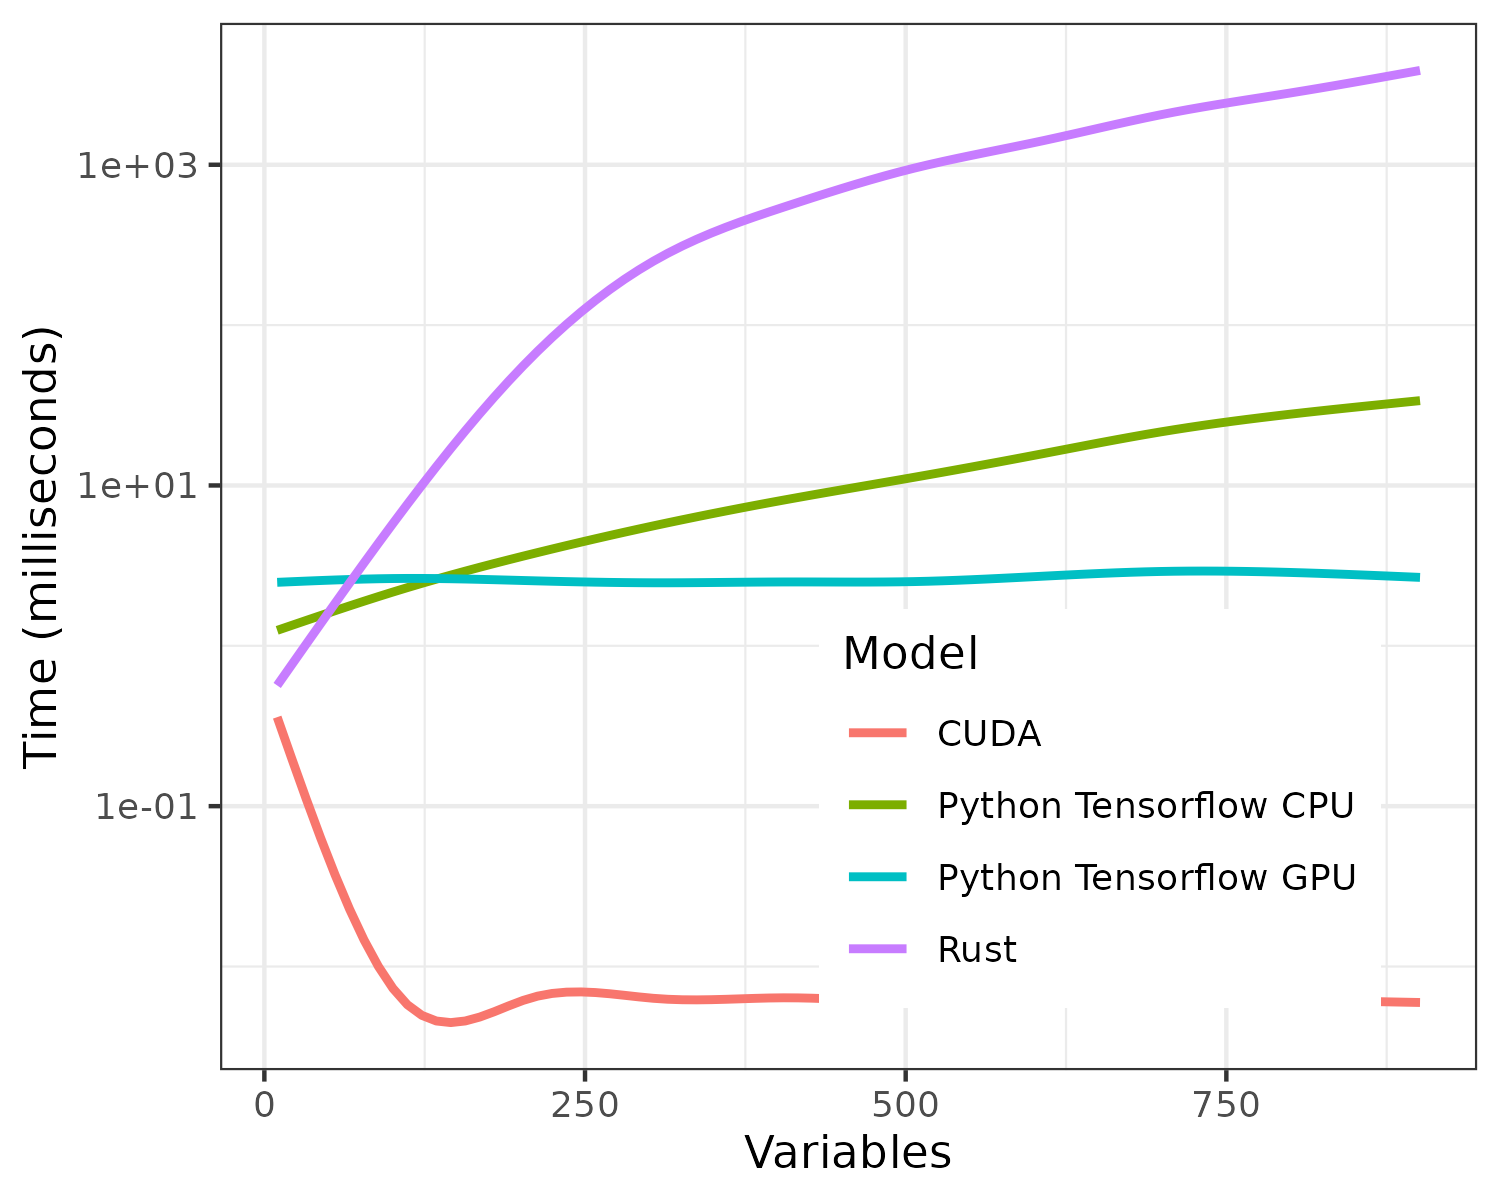
\includegraphics[width=\linewidth]{variables.png}
	\end{center}
	\caption{Average execution time related to the number of variables in the input vector. Lower time is better. Time is scaled on a $\log10$ scale to show the models relations to eachother.}
	\label{fig:graph_variables}
\end{figure}


\begin{figure}[h]
	\begin{center}
    % \includesvg[width=\linewidth]{svg/bootstraps}
		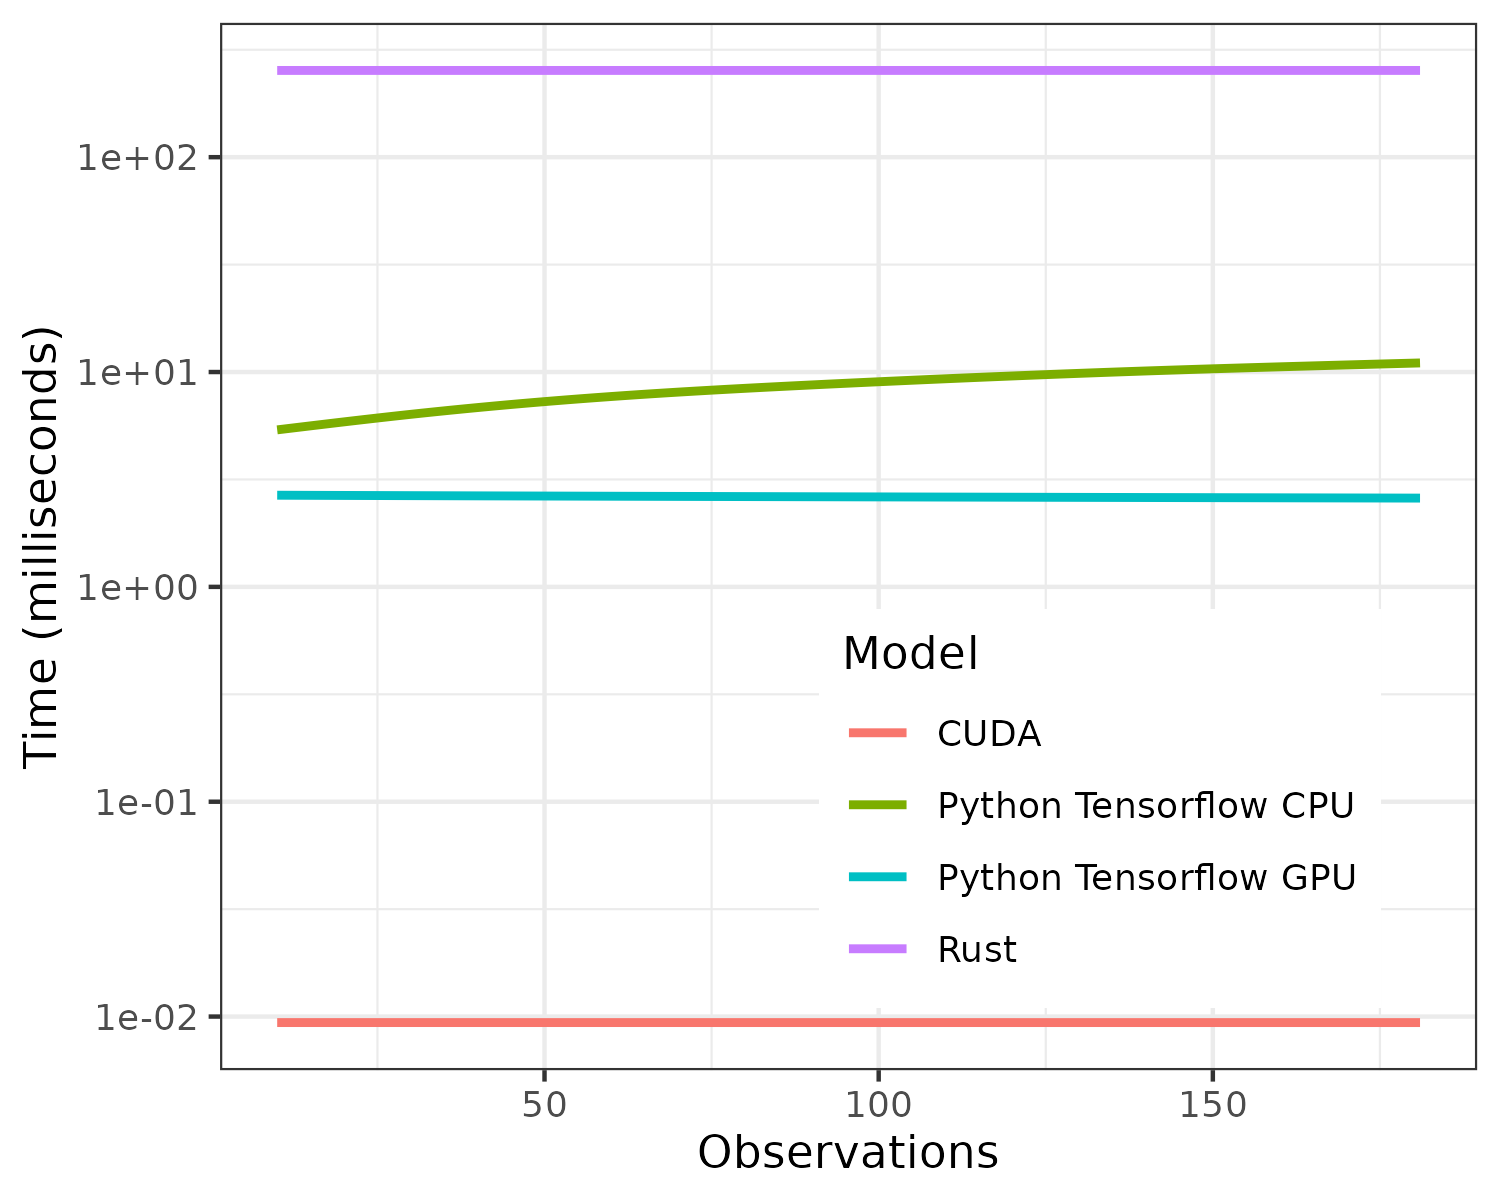
\includegraphics[width=\linewidth]{bootstraps.png}
	\end{center}
	\caption{Graph}
	\label{fig:graph_bootstraps}
\end{figure}

As with Figure \ref{fig:graph_bootstraps} and Figure \ref{fig:graph_variables}

\section{Discussion}


\section{Conclusion}

\newpage
\bibliographystyle{ieeetr}
\bibliography{refs}

\end{document}
